\documentclass[12pt]{article}
\usepackage[margin=1.2in]{geometry}
\usepackage[all]{nowidow}
\usepackage[hyperfigures=true, hidelinks, pdfhighlight=/N]{hyperref}
\usepackage{graphicx,amsmath,physics,tabto,float,amssymb,pgfplots,verbatim,tcolorbox}
\usepackage{listings,xcolor,siunitx,subfig,keyval2e,caption,import}
\numberwithin{equation}{section}
\numberwithin{figure}{section}
\definecolor{stringcolor}{HTML}{C792EA}
\definecolor{codeblue}{HTML}{2162DB}
\definecolor{commentcolor}{HTML}{4A6E46}
\lstdefinestyle{appendix}{
    basicstyle=\ttfamily\footnotesize,commentstyle=\color{commentcolor},keywordstyle=\color{codeblue},
    stringstyle=\color{stringcolor},showstringspaces=false,numbers=left,upquote=true,captionpos=t,
    abovecaptionskip=12pt,belowcaptionskip=12pt,language=Python,breaklines=true,frame=single}
\lstdefinestyle{inline}{
    basicstyle=\ttfamily\footnotesize,commentstyle=\color{commentcolor},keywordstyle=\color{codeblue},
    stringstyle=\color{stringcolor},showstringspaces=false,numbers=left,upquote=true,frame=tb,
    captionpos=b,language=Python}
\renewcommand{\lstlistingname}{Appendix}
\pgfplotsset{compat=1.17}

\title{Capacitors}
\date{\textbf{11 August 2020}}
\author{}

\begin{document}

    \begin{titlepage}
        \maketitle
        \center
        \textbf{\large{PHY2004W}}
        \textbf{\large{KDSMIL001}}
        \tableofcontents
    \end{titlepage}
    
    \section{Introduction}
    In this report we will investigate capacitors, specifically in the context of a 
    Resistor-Capacitor (RC) circuit. Firstly we will answer some questions regarding the theory 
    of capacitors and RC circuits, then we will do some experiments and investigate the effects 
    of different frequencies of AC voltage as well as different resistances on the behaviour 
    of RC circuits.

    \section{Theory Questions and Answers}
    \begin{enumerate}
        \item \textbf{Question}: How are $A$, $d$, and $\epsilon$ related, where $A$ is the area of one of the 
        plates in a capacitor, $d$ is the distance between the two plates, and $\epsilon$ is 
        the dielectric constant of the material between the plates. \newline
        \textbf{Answer}: It's fairly easy to see that an increase in the area of the plates of 
        a capacitor $A$ would result in an increase of the amount of charge each plate could hold. 
        This in turn would increase the magnitude of the electric field between each plate and thus 
        increase the potential difference between the plates when fully charged. This results in an 
        increase in capacitance. 
        Similarly the value of $\epsilon$, which is present in the equation for the electric field at 
        a point, will have an effect on the capacitance. Increasing $\epsilon$ results in a decrease 
        in $\vec{E}$ between the plates, allowing for more charge to build up on the plates. 
        Finally, the value of $d$ will also have an inversely proportional effect on the electric 
        field, meaning an increase in $d$ will lead to a decrease in $\vec{E}$ and thus a decrease in 
        the amount of charge able to build up on the plates. 
        This is all summed up in this equation for the capacitance of a capacitor:
        \begin{equation}
            C=\frac{A\epsilon}{d}
            \label{eqn:capacitance}
        \end{equation}
        

        \item \textbf{Question}: By making use of dimensional analysis show that the units of the 
        charging time of a capacitor $\tau$ as given by $\tau = RC$ is seconds (s). \newline
        \textbf{Answer}: $R$ is given by $V/I$, the dimensions of which are 
        \begin{align*}
            &\frac{M^{\frac{1}{2}}L^{\frac{1}{2}}T^{-1}}{M^{\frac{1}{2}}L^{1\frac{1}{2}}T^{-2}} \\
            \implies &L^{-1}T
        \end{align*}
        We also know that $C$ is given by $Q/V$, the dimensions of which are
        \begin{align*}
            &\frac{M^{\frac{1}{2}}L^{1\frac{1}{2}}T^{-1}}{M^{\frac{1}{2}}L^{\frac{1}{2}}T^{-1}} \\
            \implies &L \\
            \implies &[\tau]=[RC]=L^{-1}TL=T
        \end{align*}

        \item \textbf{Question}: Explain what effect an increase and decrease in frequency $\omega$ will have 
        on the reactance and therefore the impedance of the $RC$ circuit. \newline
        \textbf{Answer}: The reactance is given by 
        \begin{equation*}
            X(\omega)=\frac{1}{\omega C}
        \end{equation*}
        meaning that reactance is inversely proportional to the frequency $\omega$. We also know that 
        the impedance of an $RC$ circuit is given by $Z=R+iX(\omega)$. From this we can deduce that 
        an increase in $\omega$ will result in a decrease in $X(\omega)$ which will in turn lead to 
        the impedance being dominated more and more by $R$. As $\omega\rightarrow\infty, Z\rightarrow R$.
    \end{enumerate}

    \section{Practical Questions and Answers}
    \begin{enumerate}\addtocounter{enumi}{3}
        \item \textbf{Question}: What is the correct way to insert a capacitor into a breadboard?
        \newline
        \textbf{Answer}: The correct way to insert a capacitor is Photo C, shown below: 
        \begin{figure}[H]
            \begin{center}
               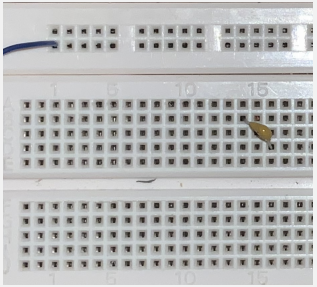
\includegraphics[scale=.5]{PhotoC.png}
               \caption{Photo C}
               \label{fig:Question4Answer}
            \end{center}
        \end{figure}
        
        The reason for this is the fact that in the other two pictures the capacitor was being short 
        circuited, once by inserting both ends into the same power rail, the long connected pieces at 
        the top and bottom, and once by inserting both ends into the same terminal strip, the shorter 
        vertical pieces.

        \item \textbf{Question}: Why does the charge on the capacitor (or the voltage across it) not 
        reach the same minimum and maximum as the applied signal in the diagram below?
        \begin{figure}[H]
            \begin{center}
               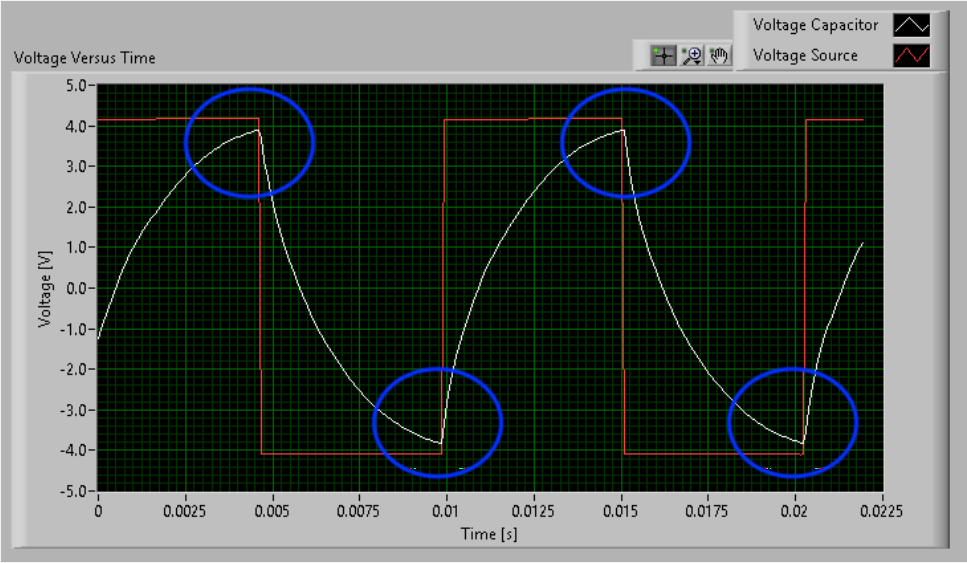
\includegraphics[scale=.5]{Question5Diagram.png}
               \caption{Voltage signal (white) across 100nF capacitor in series with 15 k$\Omega$ resistor}
               \label{fig:Question5Diagram}
            \end{center}
        \end{figure}
        What would you change to ensure the capacitor reaches the same maximum and minimum as the 
        applied signal? \newline
        \textbf{Answer}: The time it takes for a capacitor to reach its full capacity is governed by 
        $\tau = RC$. This means that in order to decrease the time it takes to charge to its theoretical 
        maximum we could decrease either the capacitance of the capacitor or the resistance of the resistor. 
        This could be done by physically changing these components, such as decreasing the surface area of 
        the plates of the capacitor, or simply by swapping out the components for those with a lower value. 
        \newline
        We could also just reduce the frequency of the applied voltage, giving the capacitor more time to 
        charge up before swapping the direction of the current, forcing it to discharge and charge up in 
        the other direction.
    \end{enumerate}

    \section{Data Collecting}
    \subsection{Resistance and Frequency Investigation}
    We were given data in the form of a text file that contained voltage measurements made by the myDAQ. 
    The myDAQ measured the voltage across the 100nF capacitor in an RC circuit as well as across the 
    function generator supplying a square wave voltage with peak-to-peak voltage of $V_{pp}=8$. This circuit 
    was set up with 5.6k$\Omega$, 8.2k$\Omega$, and 15k$\Omega$ resistors separately. Each circuit was 
    recorded with 100Hz, 200Hz, 500Hz, and 1000Hz, giving us 12 datasets to work with. This data can be 
    regarded as having a 2\% uncertainty due to the accuracy of the equipment used. We used Python to 
    interpret this data into the plots in \autoref{sec:FreqResistorResponse}, the code for which is in
    \autoref{code:FreqRes}

    \subsection{Decay Time from the Oscilloscope}
    The figure below is the screen of an oscilloscope measuring the voltage across the frequency generator 
    and the capacitor in an RC circuit with capacitance C=100nF and resistance R=5.6k$\Omega$. We want to 
    determine the time it takes for the capacitor to fully discharge, that is the time difference between 
    the capacitor being at full charge (in this case 4V) and it being at full charge in the "other direction", 
    (having -4V across it).
    \begin{figure}[H]
        \begin{center}
           \includegraphics[width=\textwidth]{Photo2.png}
           \caption{Oscilloscope Display}
           \label{fig:DecayTimeScreen}
        \end{center}
    \end{figure}
    Looking at where the blue line meets the yellow line, it seems to properly come in contact after 17 
    subdivisions, which corresponds to 3.4ms. The is an analogue measurement so it has a triangular 
    probability density function, so in order to calculate the uncertainty we use the following formula
    \begin{equation}
        u=\frac{a}{2\sqrt{6}}
    \end{equation}
    where $a$ is the difference between our best upper bound and our best lower bound for the measurement. 
    In our case our best guess could be between 3.2ms and 3.6 ms, so $a=0.4$. This gives us $u=0.081649$. 
    We also need to consider that the oscilloscope has an uncertainty of 2\%. Thus our uncertainty is 
    $\sqrt{(0.081649)^2+(2\%\cdot 3.4)^2}=0.27325$
    That gives us a final measurement of Decay Time = $3.40\pm 0.27$ms. 

    \subsection{Current Measurement}\label{sec:currentMeasurement}
    In order to investigate the phase difference between current and source voltage in an RC circuit 
    (\autoref{sec:current}) we needed to collect some data. We did this by measuring the voltage supplied 
    by the function generator, which was producing a sinusoidal signal with $V_{pp}=8$, as well as the 
    voltage across a 15k$\Omega$ resistor. This was done using the myDAQ as we did above. As before, the 
    circuit was completed with a 100nF capacitor. 

    \section{Analysis}
    \subsection{Frequency and Resistor Response}\label{sec:FreqResistorResponse}
    Apologies in advance for the small plot size but they are vectorised so you can zoom in as far as you like. 
    \begin{figure}[H]%
        \centering
        \subfloat[100Hz]{\scalebox{0.4}{\subimport{Plots}{Cap_100Hz_5k6.pgf}}}%
        \qquad
        \subfloat[200Hz]{\scalebox{0.4}{\subimport{Plots}{Cap_200Hz_5k6.pgf}}}
        \qquad
        \subfloat[500Hz]{\scalebox{0.4}{\subimport{Plots}{Cap_500Hz_5k6.pgf}}}
        \qquad
        \subfloat[1000Hz]{\scalebox{0.4}{\subimport{Plots}{Cap_1000Hz_5k6.pgf}}}
        \caption{Voltage readings for various frequencies of AC voltage across a 5.6k$\Omega$ resistor}
        \label{fig:5.6kResistor}
    \end{figure}
    
    From the figures above, it's clear to see that an increase in frequency leads to the capacitor not being 
    able to charge up fully in the given time. This makes sense as nothing else in the circuit is changing 
    so the time constant $\tau$ is remaining the same throughout as the time given to the capacitor for it 
    to charge up decreases.
    
    \begin{figure}[H]%
        \centering
        \subfloat[100Hz]{\scalebox{0.4}{\subimport{Plots}{Cap_100Hz_8k2.pgf}}}%
        \qquad
        \subfloat[200Hz]{\scalebox{0.4}{\subimport{Plots}{Cap_200Hz_8k2.pgf}}}
        \qquad
        \subfloat[500Hz]{\scalebox{0.4}{\subimport{Plots}{Cap_500Hz_8k2.pgf}}}
        \qquad
        \subfloat[1000Hz]{\scalebox{0.4}{\subimport{Plots}{Cap_1000Hz_8k2.pgf}}}
        \caption{Voltage readings for various frequencies of AC voltage across a 8.2k$\Omega$ resistor}
        \label{fig:8.2kResistor}
    \end{figure}

    The same is true for the plots above. The resistor in this circuit had a higher resistance and, as 
    we expect from the equation $\tau=RC$, the capacitor couldn't even charge fully at 200Hz, where the 
    circuit with less resistance could. \newline
    \newline
    Below in \autoref{fig:15kResistor} we see exactly the same pattern. A higher resistance leads to the 
    time constant being large and thus the capacitor cannot charge fully in the time given, with it charging 
    less and less per cycle the higher the frequency of the applied voltage.
    
    \begin{figure}[H]%
        \centering
        \subfloat[100Hz]{\scalebox{0.4}{\subimport{Plots}{Cap_100Hz_15k.pgf}}}%
        \qquad
        \subfloat[200Hz]{\scalebox{0.4}{\subimport{Plots}{Cap_200Hz_15k.pgf}}}
        \qquad
        \subfloat[500Hz]{\scalebox{0.4}{\subimport{Plots}{Cap_500Hz_15k.pgf}}}
        \qquad
        \subfloat[1000Hz]{\scalebox{0.4}{\subimport{Plots}{Cap_1000Hz_15k.pgf}}}
        \caption{Voltage readings for various frequencies of AC voltage across a 15k$\Omega$ resistor}
        \label{fig:15kResistor}
    \end{figure}\noindent
    All of these plots were created using the code in \autoref{code:FreqRes}

    \subsection{Time Constant \texorpdfstring{$\tau=RC$}{t=RC}}
    In this section we will try to experimentally determine the value of the time constant for two RC circuits 
    with C = 100nF and R = 15k$\Omega$ and 5.6k$\Omega$ respectively. To do this, we will look at the equations 
    that describe the charging and discharging of a capacitor:
    \begin{align}
        \text{Charging:}\hspace{15pt} V_C(t)&=V_\epsilon[1-e^{-\frac{t}{RC}}] \label{eqn:CapCharging}\\
        \text{Discharging:}\hspace{15pt} V_C(t)&=V_\epsilon e^{-\frac{t}{RC}} \label{eqn:CapDischarging}
    \end{align}
    By linearising these equations we get the following
    \begin{align}
        \text{Charging:}\hspace{15pt} &\ln(V_\epsilon-V_C)=-\frac{t}{RC}+\ln(V\epsilon) \label{eqn:CapChargingLinearised}\\
        \text{Discharging:}\hspace{15pt} &\ln(V_C)=-\frac{t}{RC}+\ln(V\epsilon) \label{eqn:CapDischargingLinearised}
    \end{align}
    Now we need to take the values from our collected data and plot, in the first case $\ln(V_\epsilon-V_C)$ 
    against $t$ and in the second case $\ln(V_C)$ against $t$. We can then perform a linear least squares fit 
    on this data to determine the slope, which will give us a value for $-\frac{1}{RC}$, from which we can extract the
    value of $\tau$. Below are the results. \newline \newline
    Starting with the 5.6k$\Omega$ resistor (\autoref{fig:DeterminingTau5k6}), our expected value is 
    \begin{equation*}
        \tau=RC=5600\times \num{1e-7}=\num{5.6e-4}
    \end{equation*}
    When we find $\tau$ for the charging and discharging plots and take their average we get a value of 
    $\tau=\num{5.7230225e-4}$. The uncertainty on this measurement starts as a standard uncertainty for 
    the line of best fit parameters and through propagation of uncertainties for the inversion and averaging 
    out we get a final value of $\tau = \num{5.7230e-4}\pm\num{0.0309e-4}$. This is quite close to our expected 
    value but does not agree within experimental uncertainty. The reason for this is likely only using 
    one charging/discharging cycle to run the analysis on. 
    \begin{figure}[H]%
        \centering
        \subfloat[Charging]{\scalebox{0.45}{\subimport{Plots}{Cap_100Hz_5k6_Charging.pgf}}}
        \qquad
        \subfloat[Discharging]{\scalebox{0.45}{\subimport{Plots}{Cap_100Hz_5k6_Discharging.pgf}}}
        \caption{5.6k$\Omega$ at 100Hz}
        \label{fig:DeterminingTau5k6}
    \end{figure}\noindent
    For the 15k$\Omega$ resistor (\autoref{fig:DeterminingTau15k}) our expected value is 
    \begin{equation*}
        \tau=RC=15000\times\num{1e-7}=\num{1.5e-3}
    \end{equation*}
    Performing exactly the same operations as above, we find $\tau=\num{1.5562e-3}\pm\num{0.0058e-3}$. Again 
    this is fairly close but does not agree within experimental uncertainty. This is likely for the same reason: 
    only using one charging/discharging cycle. All of the code for this section is in \autoref{code:DeterminingTau}
    \begin{figure}[H]%
        \centering
        \subfloat[Charging]{\scalebox{0.45}{\subimport{Plots}{Cap_100Hz_15k_Charging.pgf}}}
        \qquad
        \subfloat[Discharging]{\scalebox{0.45}{\subimport{Plots}{Cap_100Hz_15k_Discharging.pgf}}}
        \caption{15k$\Omega$ at 100Hz}
        \label{fig:DeterminingTau15k}
    \end{figure}

    \subsection{Phase Difference Between Current \texorpdfstring{$I$}{I} and Source Voltage \texorpdfstring{$V_\epsilon$}{Ve} in an RC Circuit}\label{sec:current}
    We will now investigate the phase difference between Current $I$ and Source Voltage $V_\epsilon$ in an RC 
    circuit. To do this we will use the data collected in \autoref{sec:currentMeasurement}. Below is the plot 
    of the source voltage and the voltage across the resistor. We aren't displaying the current as it is 
    minuscule compared to the source voltage, but the voltage will have the same period and phase difference.
    \begin{figure}[H]
        \begin{center}
           \scalebox{.6}{\subimport{Plots}{Res_100Hz_15k.pgf}}
           \caption{Voltage across a 15k$\Omega$ resistor in an RC circuit and the applied AC voltage}
           \label{fig:CurrentPhaseDiff}
        \end{center}
    \end{figure}
    We used the function \texttt{scipy.signal.find\_peaks} to find the positions of the maxima of both 
    sets of data. We could then calculate the average time difference between peaks and found it to be 
    exactly $0.001077$. There was originally an uncertainty on this value but it turned out to be 
    due to rounding errors in \texttt{float64} precision when calculating the standard deviation 
    with \texttt{numpy.std}. However there \textit{must} be some uncertainty to this measurement and since 
    we didn't include the uncertainty due to the inaccuracy of the equipment used since we took an average, 
    we'll use that for this. That gives us a difference in phase of $0.001077\pm 0.000022$ seconds. Taking 
    the wavelength into account ($0.00992267\pm 0.00000019$), we can get a value in radians, namely 
    $0.2170788\pi \pm 0.0000042$. All of the code for this section is in \autoref{code:current}

    \subsection{Capacitance C}
    In this section we will verify the capacitance C of the capacitor used in this experiment. To do this 
    we will derive an equation for C from the equation describing the discharging of a capacitor $V_{C} = V_\epsilon e^{-\frac{t}{RC}}$:
    \begin{align*}
        V_{C1} &= V_\epsilon e^{-\frac{t_1}{RC}} \\
        V_\epsilon &= V_{C2}e^{\frac{t_2}{RC}} \\
        \therefore V_{C1} &=  V_{C2}e^{\frac{t_2}{RC}}e^{-\frac{t_1}{RC}} \\
        &=V_{C2}e^{\frac{t_2-t_1}{RC}} \\
        \implies \frac{V_{C1}}{V_{C2}} &= e^{\frac{t_2-t_1}{RC}} \\
        \implies \log_e(\frac{V_{C1}}{V_{C2}}) &= \frac{t_2-t_1}{RC} \\
        \implies C &= \frac{t_2-t_1}{R\log_e(\frac{V_{C1}}{V_{C2}})}
    \end{align*}
    This would be valid if the discharging started at $V_C=0$, but ours starts at $V_C=4$ so we must adjust 
    this equation, leaving us with
    \begin{equation}
        C = \frac{t_2-t_1}{R\log_e(\frac{V_{C1}+4}{V_{C2}+4})}
        \label{eqn:capacitanceExperimental}
    \end{equation}
    Calculating this using two reasonably chosen points we get 
    \begin{align*}
        t_1&=0.005692, V_{C1}=-0.5 \\
        t_2&=0.007307, V_{C2}=-3.9 \\
        \therefore C&= \num{8.111522479e-8} \text{F}
    \end{align*}
    Now we need to consider the uncertainty of this measurement. It's a complicated one but if we break it 
    down we see that uncertainties come from the measurement of the time and voltage for each point, which 
    is 2\% of the value as that's the accuracy of the equipment used in this experiment. Then the logarithm 
    needs to be considered, as well as the final division. Note that there is no uncertainty on the value 
    of the resistor as we know it to be 5.6k$\Omega$. Below are each of the separate uncertainties as well 
    as the final.
    \begin{alignat*}{2}
        t_2-t_1 &=\num{1.615e-3}\pm \num{0.1852469843e-3} &&: \text{Type B, Addition Propagation}\\
        \log_e(\frac{V_{C1}+4}{V_{C2}+4})&=3.555348061\pm 0.7800052328 &&: \text{Type B, Function Propagation}\\
        R\log_e(\frac{V_{C1}+4}{V_{C2}+4})&=19909.94914 \pm 4369.029304 &&: \text{Multiplication by a Constant}\\
        C&= \num{8.111522479e-8} \pm \num{2.008132925e-8} &&: \text{Division Propagation}
    \end{alignat*}
    and so our final result is $C= \num{8.112e-8}\pm\num{2.008e-8}$F, which agrees with our expected 
    result of 100nF or $\num{10e-8}$F.

    \section{Conclusion and Recommendations}
    To conclude, in many respects these experiments were successful. We investigated the relationship 
    between resistor value in an RC circuit and the frequency of the AC voltage supplied to it and found 
    that the resistance has a proportional effect on the time constant $\tau$ of the circuit, as we would 
    expect from the equation $\tau=RC$. \newline
    We determined the time constant $\tau$ in its own right for two set-ups of RC circuit and found them 
    to be close to, but not in agreement within experimental uncertainty with, the relevant expected values.
    This disagreement could likely be avoided in future experiments by taking data from multiple charging/discharging 
    cycles to analyse. \newline
    We investigated the phase difference between current and source voltage in an RC circuit and found it 
    to be around $\frac{\pi}{5}$. \newline
    Finally we verified that the capacitance in our circuit was in fact (around) 100nF by using equations 
    that describe the discharging of a capacitor in an RC circuit. Our experimentally determined value 
    agreed with the expected value but the uncertainty could likely be greatly improved by using more than 
    one set of points and averaging the final value.

    \newpage
    \section{Appendix}
    \setcounter{figure}{0} \renewcommand{\thefigure}{A.\arabic{figure}}
    \lstinputlisting[caption=Code that interprets Resistance Frequency data, style=appendix, label=code:FreqRes]{FrequencyResistance.py}
    \lstinputlisting[caption=Code that determines $\tau$ from charging and discharging data, style=appendix, label=code:DeterminingTau]{DeterminingTau.py}
    \lstinputlisting[caption=Code that interprets Current data, style=appendix, label=code:current]{Current.py}
    
\end{document}